\documentclass[aspectratio=169, 10pt, utf8, mathserif]{beamer}
%导言区
\usepackage{ctex}
\usepackage{amsmath, amsfonts, amssymb, amsthm}
\usepackage{graphicx}
\usepackage{fontspec}
\usepackage{ulem} %解决下划线换行紊乱
\usepackage{caption} %添加图、表的标题
\usepackage{subfigure}
\usepackage{theorem}
\usepackage[backend=bibtex,sorting=none]{biblatex} %不列出所有作者
%\usepackage[backend=bibtex,sorting=none,maxnames=9,minnames=3]{biblatex} %列出所有作者,具体选择列不列可以由其前的“%”来决定
\addbibresource{ref.bib} %BibTeX数据文件及位置
\setbeamerfont{footnote}{size=\tiny} %设置脚注引用文献的字体大小
%\setbeamertemplate{bibliography item}[text] %设置参考文献图标样式数字标号
\usepackage{appendix} %增加附录
\usepackage{multicol} %分栏
\usepackage{syntonly} %只编译文件是否成功,省时省力
%\syntaxonly %不注释代表只编译是否成功
%\usepackage[marginal]{footmisc} %首页添加脚注无缩进
%\renewcommand{\thefootnote}{} %首页添加脚注无编号
\usepackage{enumerate}
\usepackage{listings} %代码包
\usepackage{xcolor} %代码高亮包
\definecolor{jnucolor}{RGB}{48, 127, 142}
\lstset{
	language=Matlab, %代码语言使用的是matlab
	%frame=shadowbox, %把代码用带有阴影的框圈起来
	%rulesepcolor=\color{red!20!green!20!blue!20}, %代码块边框为淡青色
	keywordstyle=\color{blue}\bfseries, %代码关键字的颜色为蓝色,粗体
	commentstyle=\color{orange}\ttfamily, %设置代码注释的颜色,原字体样式\textit
	backgroundcolor=\color{darkgray!6}, %背景色
	showstringspaces=false, %不显示代码字符串中间的空格标记
	numbers=left, %显示行号
	numberstyle=\tiny, %行号字体
	basicstyle=\ttfamily,
	stringstyle=\ttfamily, %代码字符串的特殊格式
	breaklines=true, %过长的代码自动换行
	extendedchars=false,  %解决代码跨页时,章节标题,页眉等汉字不显示的问题
	escapebegin=\begin{CJK*}{GBK}{hei},escapeend=\end{CJK*} %防止中文报错
	texcl=true,
	morekeywords={classdef,function,global,parfor,persistent,spmd,plot}} %设置更多关键词

%使用的主题样式和主题色
%\usetheme{Antibes}
%\usetheme{Marburg} % TOC tab 
%\usetheme{Berkeley} 
%\usetheme{PaloAlto} 
%\usetheme{Goettingen} 
%\usetheme{Hannover}  % ok2 
%\usetheme{Antibes}  % Tree 
%\usetheme{JuanLesPins}  % ok 3 
%\usetheme{Montpellier} 
%\usetheme{Bergen}   % w/o guide 
%\usetheme{boxes} 
%\usetheme{Bergen} 
%\usetheme{Madrid} 
%\usetheme{Pittsburgh} 
%\usetheme{Rochester} 
\usetheme{Berlin}   % mini guide 
%\usetheme{Ilmenau}   %ok 4 
%\usetheme{Dresden} 
%\usetheme{Darmstadt}   %ok 1 
%\usetheme{Frankfurt} 
%\usetheme{Singapore}  % ok ok 
%\usetheme{Szeged} % ok ok ok 
%\usetheme{Copenhagen} 
%\usetheme{Luebeck} 
%\usetheme{Malmoe} 
%\usetheme{Warsaw} 
%\usecolortheme{beaver} 
%\usecolortheme{albatross} %深蓝色
%\usecolortheme{beetle} %蓝灰色
%\usecolortheme{dove} 
%\usecolortheme{fly} 
%\usecolortheme{seagull} 
%\usecolortheme{crane} 
%\usecolortheme{rose} 
%\usecolortheme{lily}   % inner color 
%\usecolortheme{orchid} % inner color 
%\usecolortheme{whale}  % outer color %深蓝色
%\usecolortheme{seahorse} % outer color    %% ok 浅紫色
%\usecolortheme{sidebartab} %浅紫色
%\usecolortheme{dolphin}  % ok ok
\usecolortheme{jnucolor} %暨大校徽的颜色

\usefonttheme{serif} %已有的字体default professionalfonts serif structurebold structureitalicserif structuresmallcapsserif

% 设置用acrobat打开就会全屏显示
\hypersetup{pdfpagemode=FullScreen}

% 设置logo
\pgfdeclareimage[height=1.3cm]{university-logo}{logo} %需提前将logo文件放到`.tex`文件中。
\logo{\pgfuseimage{university-logo}}

\usepackage{listings}
\usepackage{xcolor} 


\definecolor{mygreen}{rgb}{0,0.6,0}
\definecolor{mygray}{rgb}{0.5,0.5,0.5}
\definecolor{mymauve}{rgb}{0.58,0,0.82}
\lstset{ %
	backgroundcolor=\color{white},   % choose the background color
	basicstyle=\footnotesize\ttfamily,        % size of fonts used for the code
	columns=fullflexible,
	breaklines=true,                 % automatic line breaking only at whitespace
	captionpos=b,                    % sets the caption-position to bottom
	tabsize=4,
	commentstyle=\color{mygreen},    % comment style
	escapeinside={\%*}{*)},          % if you want to add LaTeX within your code
	keywordstyle=\color{blue},       % keyword style
	stringstyle=\color{mymauve}\ttfamily,     % string literal style
	frame=shadowbox,
	rulesepcolor=\color{red!20!green!20!blue!20},
	% identifierstyle=\color{red},
	numbers=left, 
	numberstyle=\tiny,
	% escapeinside=' ',
	xleftmargin=2em,
	xrightmargin=2em, 
	aboveskip=1em
}

%-------------开始-------------------
\begin{document}
	
	%每个章节都有小目录
	\AtBeginSection[]
	{
		\begin{frame}
			\frametitle{目录}
			\zihao{4}
				\tableofcontents[currentsection]
			
		\end{frame}
	}
	
	\title{基于GRU的股市预测}

	\author[余思贤]{\zihao{4}组长:苏日清\\ \zihao{5}
		组员:余思贤,谭铭濠,梁宗威
		\quad \\ \vspace{0.5cm}  \quad\zihao{6}{ }}
	\institute[ ]
	{
		 
	}
	\date{\today}
	%显示封面页
	\begin{frame}
		%\maketitle
		\titlepage
	\end{frame}
	
%	\begin{frame}
%		\frametitle{目录}
%		\begin{multicols}{2}
%			\tableofcontents[hideallsubsections]
%		\end{multicols}
%		%\tableofcontents[hideallsubsections]
%	\end{frame}
	
\section{课程设计的任务与要求}


	\begin{frame}
		\frametitle{课程设计的任务}
		\zihao{3}
\begin{enumerate}
	\item 熟悉MATLAB中深度学习工具箱的使用方法,喂入数据的方法,配置训练的方法,保存模型的方法和调用模型的方法;
	\item 能画出学习模型的基本框架,理解其基本原理;
	\item 基于GRU对中国石化的开盘股价进行预测。
\end{enumerate}
	\end{frame}

\begin{frame}
	\frametitle{课程设计的要求}
	\begin{enumerate}
		\zihao{3}
		\item 学会MATLAB软件的安装;
		\item 熟练掌握MATLAB的使用,掌握深度学习工具箱的使用;
		\item 能使用深度学习工具箱根据需求搭建神经网络,喂入数据,训练,得出模型并能调用;
		\item 通过调参使得模型能更好的贴合实际,打到更好的效果。
	\end{enumerate}
\end{frame}	
\section{研究基础}
\begin{frame}
	\frametitle{序列数据神经网络}
	循环神经网络(Recurrent Neural Network,RNN)是一种用于处理序列数据的神经网络。相比一般的神经网络来说,他能够处理序列变化的数据。比如某个单词的意思会因为上文提到的内容不同而有不同的含义,RNN就能够很好地解决这类问题。
	
	一般来说,普通RNN网络形式如下:
	\begin{align}
		h^{\prime}=&\delta(w_h h+w_i x+b^{h})\\
		y=&\delta( w_o h^{\prime}+b^{y})
	\end{align}
	
	
	其中$ h^{\prime} $为传入下一节点的参数,$ y $常使用对$ h^{\prime} $进行唯独映射,然后使用$ softmax $进行分类得到所需的参数。
\end{frame}	
\begin{frame}
	\frametitle{序列数据神经网络}
	\begin{figure}[H]
		\centering
		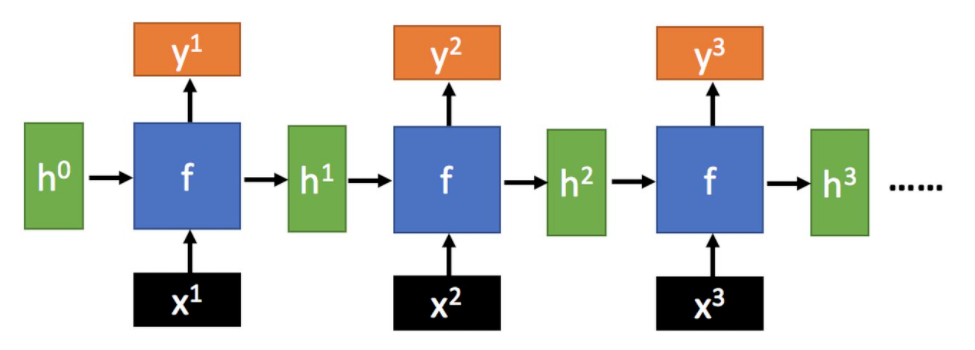
\includegraphics[width=\linewidth]{pic/screenshot001}
		\caption{多级RNN网络构成}
		\label{fig:screenshot001}
	\end{figure}
\end{frame}	
\begin{frame}
	\frametitle{LSTM结构}
	长短期记忆(Long short-term memory, LSTM)是一种特殊的RNN,主要是为了解决长序列训练过程中的梯度消失和梯度爆炸问题。简单来说,就是相比普通的RNN,LSTM能够在更长的序列中有更好的表现。
	LSTM网络的表达式如下:
	\begin{align}
		c^t=&z^f\odot c^{t-1}+z^{i}\odot z\\
		h^{t}=&z^{o}\odot \tanh{c^{t}}\\
		y^{t}=&\delta(W^{\prime}h^{t}+b^{y})
	\end{align}
其中$ c^{t} $可以理解为长期记忆,主要是用来保存节点传递下来的数据的,每次传递会对某些维度进行“忘记”并且会加入当前节点所包含的内容;,$ h^{t} $则为短期记忆,仅保存了先前节点的信息。
\end{frame}	
\begin{frame}
	\frametitle{LSTM结构}
	\begin{figure}[H]
		\centering
		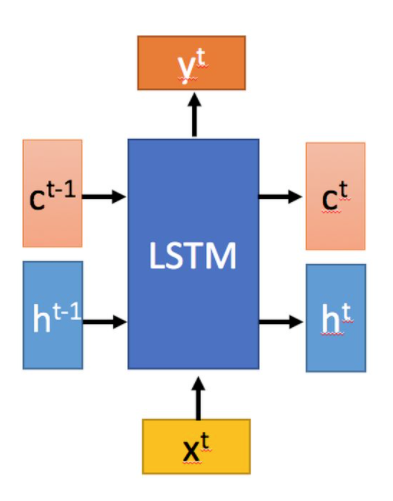
\includegraphics[width=0.3\linewidth]{pic/screenshot002}
		\caption{LTSM网络结构}
		\label{fig:screenshot002}
	\end{figure}
\end{frame}	
\begin{frame}
	\frametitle{GRU网络}
	GRU(Gate Recurrent Unit)是循环神经网络(Recurrent Neural Network, RNN)的一种。和LSTM(Long-Short Term Memory)一样,也是为了解决长期记忆和反向传播中的梯度等问题而提出来的。
	
	GRU的输入输出结构与普通的RNN是一样的。
	
	其表达式为:
	\begin{align}
		r^{t}=&\delta(x^{t}w^{xr}+h^{t-1}w^{hr}+b^{r})\\
		z^{t}=&\delta(x^{t}w^{xz}+h^{t-1}w^{hz}+b^{z})\\
		h^{\prime}=&\tanh{x^{t}w^{xr}+r^{t}\odot h^{t-1}w^{hh}+b^{h} }\\
		h^t=&(1-z)\odot h^{\prime}+z\odot h^{t-1}\\
		y^{t}=&\text{softmax}(h^{t}w^{hy}+b^{y})
	\end{align}
\end{frame}	
\begin{frame}
	\frametitle{GRU网络}
	GRU与LSTM相比,需要训练的参数较少,但也能达到与LSTM相近的效果。其训练的参数少,对硬件要求要求较低,因此本文采用GRU进行实现
	\begin{figure}[H]
		\centering
		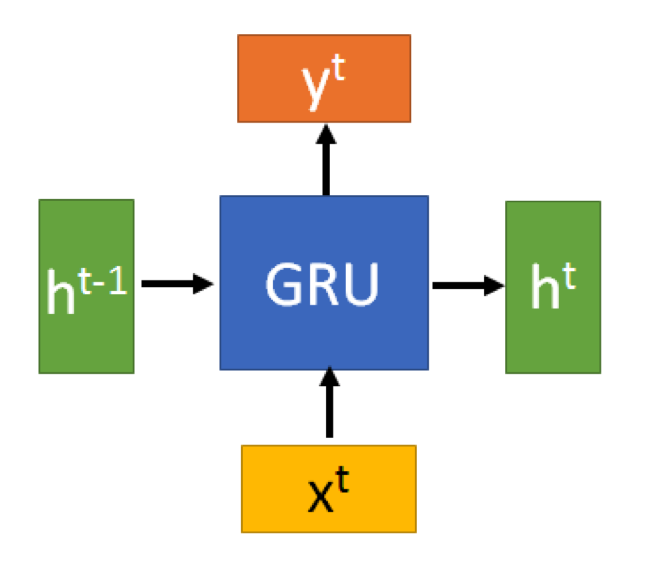
\includegraphics[width=0.3\linewidth]{pic/screenshot003}
		\caption{GRU的输入输出结构}
		\label{fig:screenshot003}
	\end{figure}
\end{frame}	
\section{训练数据的准备}
\begin{frame}
	\frametitle{数据采集}
	这里使用Python爬取近16年中国石化(600028)的股市信息。
	
	代码如下:
	\begin{figure}[H]
		\centering
		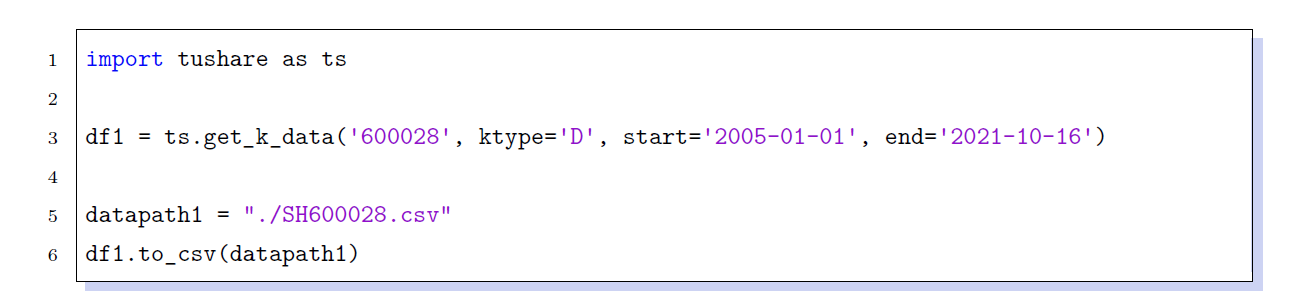
\includegraphics[width=1\linewidth]{pic/screenshot032}
		\label{fig:screenshot032}
	\end{figure}
	
得到了4032行数据,包括:时间、开盘价格、收市价、高位、低位、成交量以及股票代码。
\end{frame}	
\begin{frame}
	\frametitle{数据处理}
	为使得模型更快收敛,并提高其准确性,对取得的数据进行归一化处理,公式如下:
	
	\begin{equation}
		x^*=\frac{X-X_{min}}{X_{max}-X_{min}}
	\end{equation}
\begin{figure}[H]
	\centering
	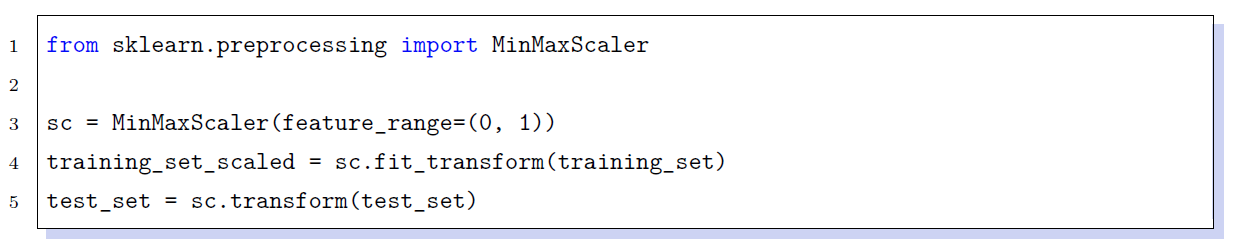
\includegraphics[width=1\linewidth]{pic/screenshot033}
	\label{fig:screenshot033}
\end{figure}

\end{frame}	
\begin{frame}
	\frametitle{数据标注}
	为了实现股票预测,需要对训练用的数据进行标注。
	
	GRU是根据过去预测未来,因此采用前两个月的数据进行对当日开盘价的预测。
	
	取出后200日的数据作为测试数据,前3832日数据作为训练数据。
	
	使用Python进行数据标注,并保存为txt文件,方便在MATLAB中进行读取调用。
	
	标注核心代码如下:
	\begin{figure}[H]
		\centering
		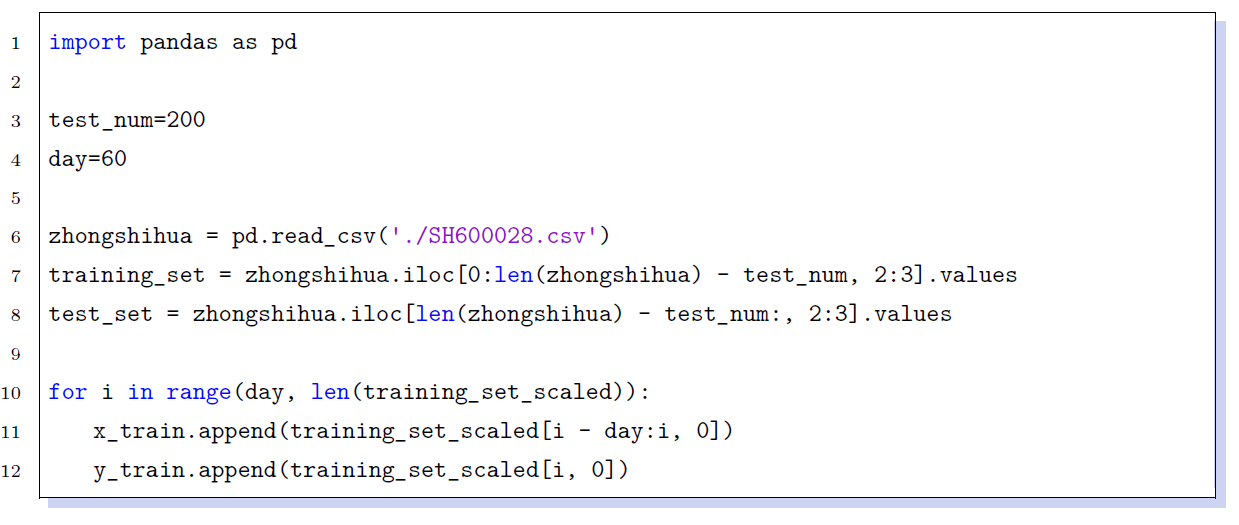
\includegraphics[width=0.7\linewidth]{pic/screenshot034}
		\label{fig:screenshot034}
	\end{figure}
	
\end{frame}	

\begin{frame}
	\frametitle{股市预测的Python实现}
	先在Python中调用tensorflow框架进行本项目的实现,验证其可行性。
	\begin{figure}[H]
		\centering
		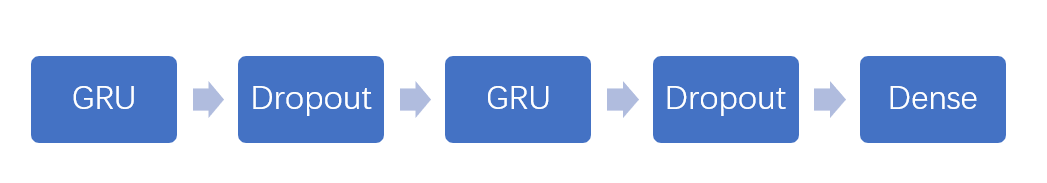
\includegraphics[width=1\linewidth]{pic/screenshot004}
		\caption{股市预测网络结构}
		\label{fig:screenshot004}
	\end{figure}
\end{frame}	
\begin{frame}
	\frametitle{股市预测的Python实现}
	核心代码如下(仅展示模型部分):
	\begin{figure}[H]
		\centering
		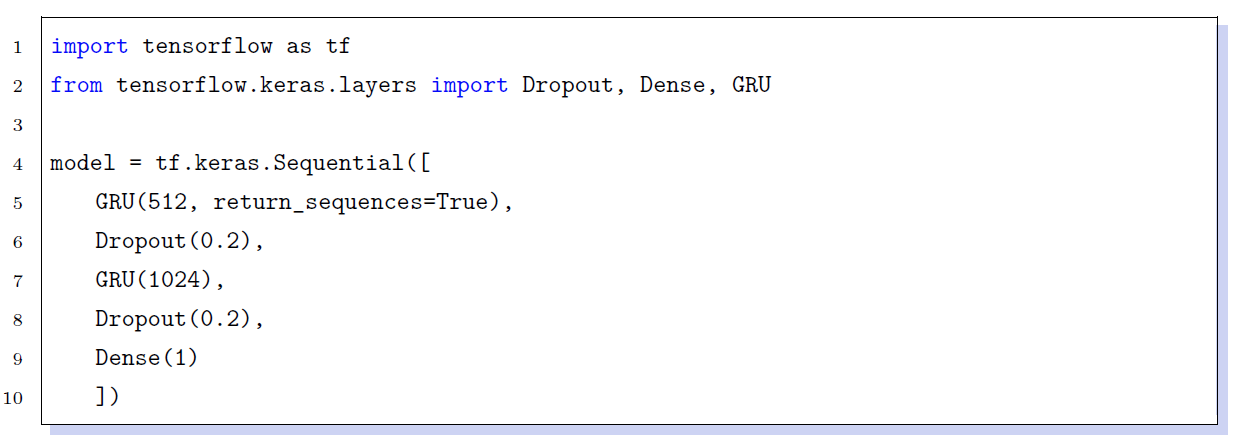
\includegraphics[width=1\linewidth]{pic/screenshot035}
		\label{fig:screenshot035}
	\end{figure}
	
\end{frame}	
\begin{frame}
	\frametitle{股市预测的Python实现}
	 
	 第一层GRU:512个单元,每次返回$ h^t $参数;
	令其中20\%的单元休眠;
	第二层GRU:1024个单元,仅最后一次返回$ h^t $参数;
	令其中20\%的单元休眠;
	最后进行全链接输出。
	
	在epochs=100,batch size=32的训练条件下,预测结果如图\ref{fig:screenshot005}:
	\begin{figure}[H]
		\centering
		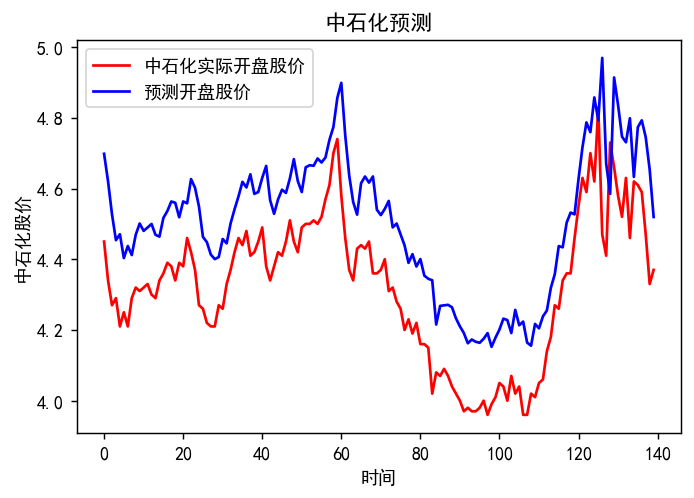
\includegraphics[width=0.4\linewidth]{pic/screenshot005}
		\caption{预测结果}
		\label{fig:screenshot005}
	\end{figure}
	
	可以看到:预测出的趋势与实际相比是较为准确的。
\end{frame}	
\section{股市预测的MATLAB实现}
\begin{frame}
	\frametitle{深度学习工具箱}
	\zihao{4}
	深度学习工具箱提供了一个用于通过算法、预训练模型和 App 来设计和实现深度神经网络的框架。在深度学习工具箱中可以使用卷积神经网络(ConvNet、CNN)和长短期记忆 (LSTM) 网络对图像、时序和文本数据执行分类和回归。可以使用自动微分、自定义训练循环和共享权重来构建网络架构,如生成对抗网络 (GAN) 和孪生网络。使用深度网络设计器,能够以图形方式设计、分析和训练网络。试验管理器可管理多个深度学习试验,跟踪训练参数,分析结果,并比较不同试验的代码。可以可视化层激活,并以图形方式监控训练进度。
\end{frame}	
\begin{frame}
	\frametitle{在MATLAB中搭建GRU神经网络}
	在深度学习工具箱中,可以快速搭建神经网络
	\begin{figure}[H]
		\centering
		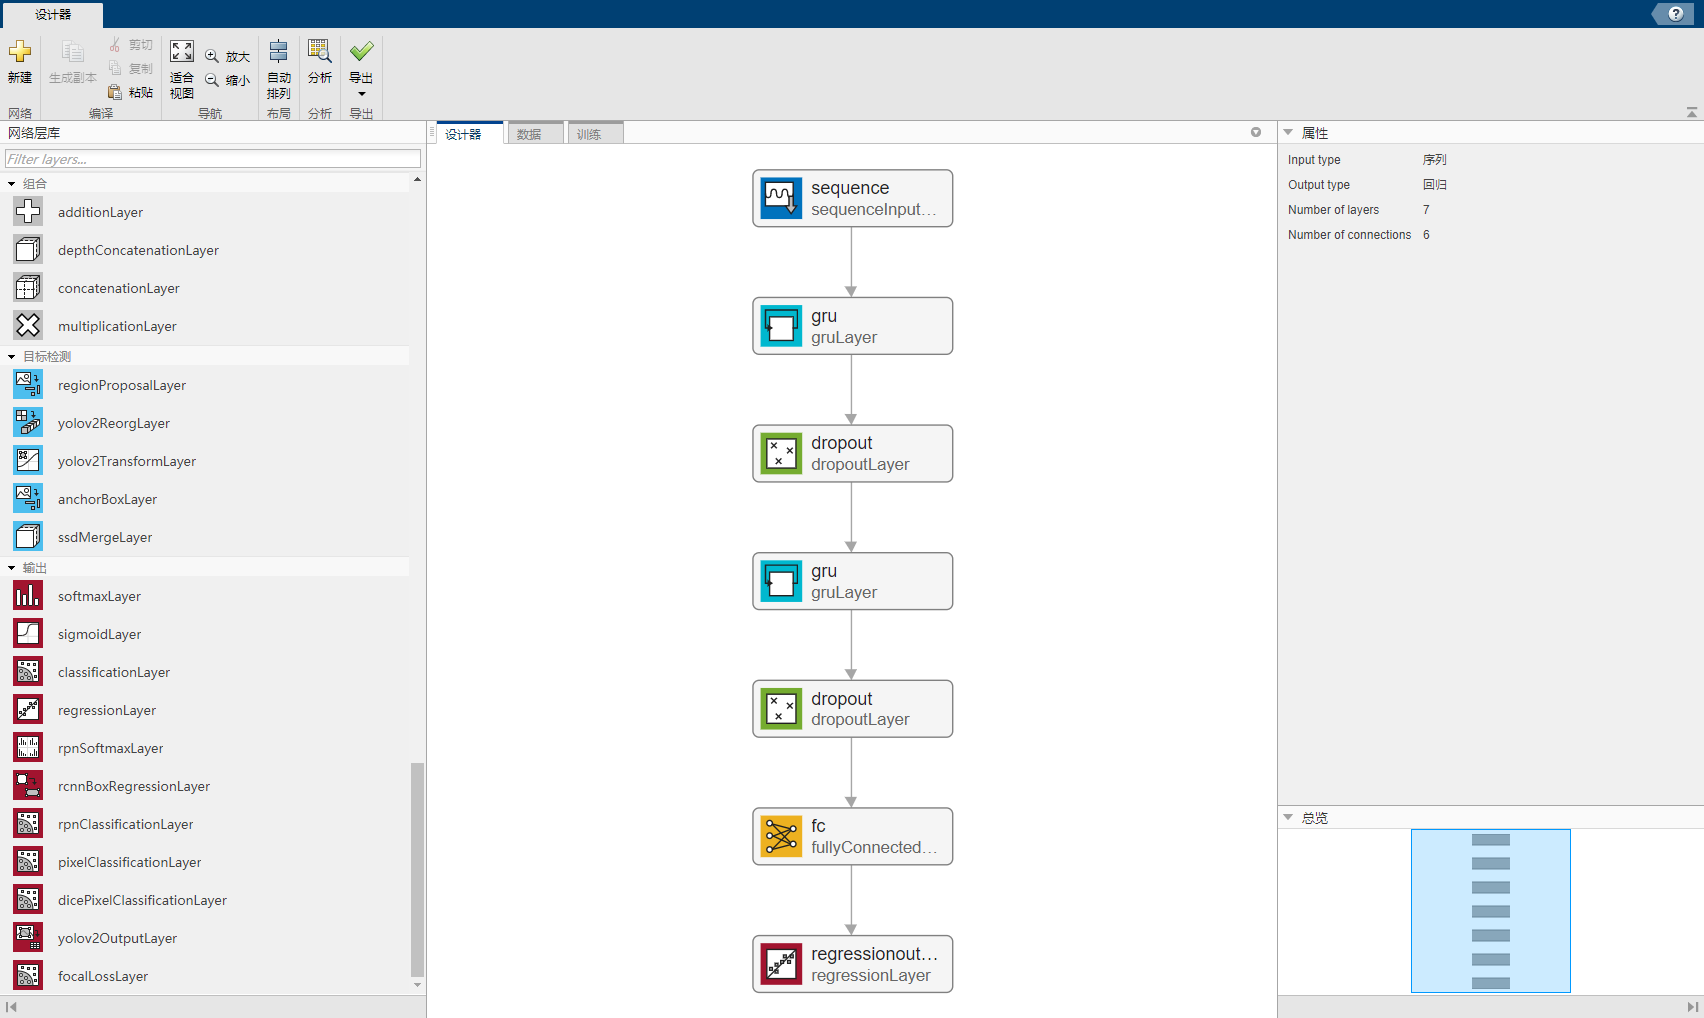
\includegraphics[width=0.7\linewidth]{pic/screenshot018}
		\caption{使用深度学习工具箱中快速搭建基础神经网络}
		\label{fig:screenshot017}
	\end{figure}
\end{frame}	
\begin{frame}
	\frametitle{在MATLAB中搭建GRU神经网络}
	通过深度学习工具箱,我们可以快速导出神经网络模型,得到结果如图\ref{fig:screenshot019}所示:
	\begin{figure}[H]
		\centering
		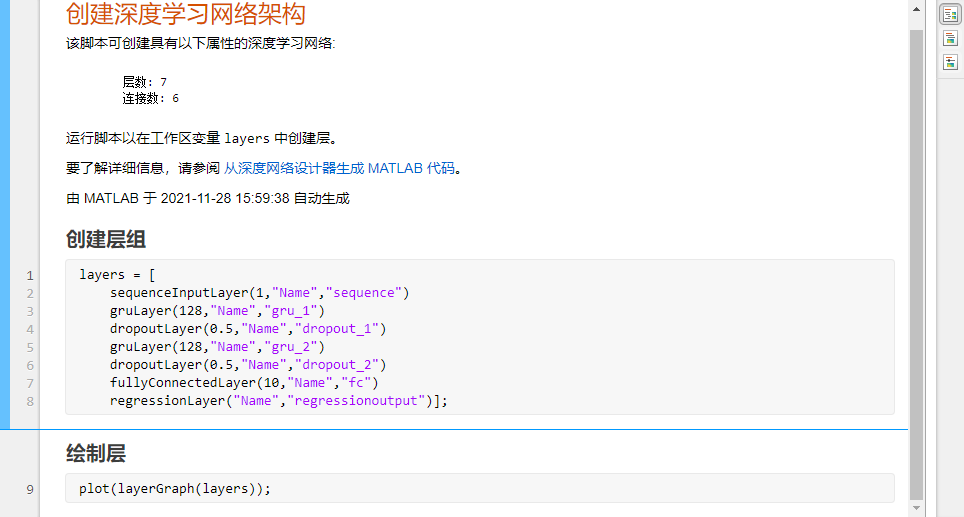
\includegraphics[width=0.6\linewidth]{pic/screenshot019}
		\caption{使用深度学习工具箱创建深度学习网络架构}
		\label{fig:screenshot019}
	\end{figure}
\end{frame}	
\begin{frame}
	\frametitle{在MATLAB中搭建GRU神经网络}
	在Matlab中,程序核心代码如下:
	
	网络架构部分:
	\begin{figure}[H]
		\centering
		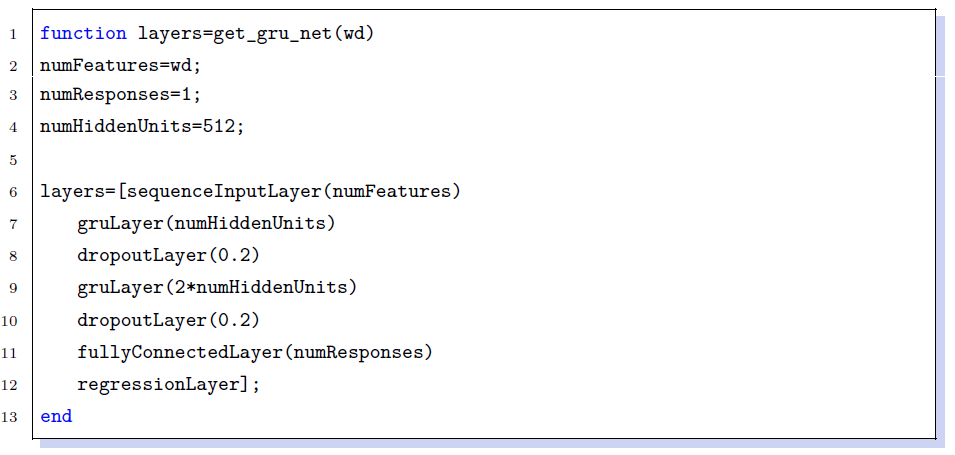
\includegraphics[width=0.7\linewidth]{pic/screenshot037}
		
		\label{fig:screenshot037}
	\end{figure}
\end{frame}	
\begin{frame}
	\frametitle{在MATLAB中搭建GRU神经网络}
	在Matlab中,程序核心代码如下:
	
	模型超参数选项设置部分:
	\begin{figure}[H]
		\centering
		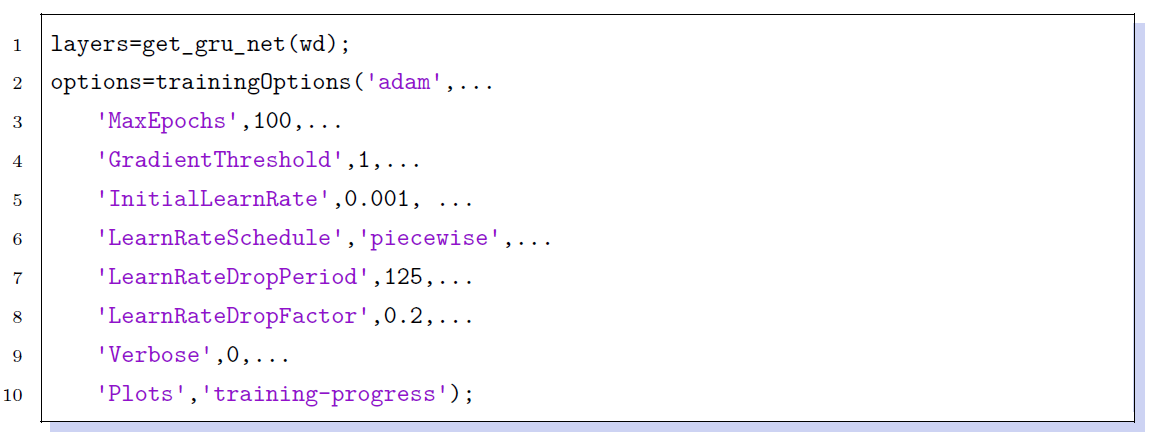
\includegraphics[width=0.7\linewidth]{pic/screenshot036}
		
		\label{fig:screenshot036}
	\end{figure}
\end{frame}	

\begin{frame}
	\frametitle{喂入数据并训练}
	在Matlab中,使用函数$ trainNetwork $将数据喂入神经网络并训练。训练过程如图\ref{fig:screenshot015}所示:
	
	\begin{figure}[H]
		\centering
		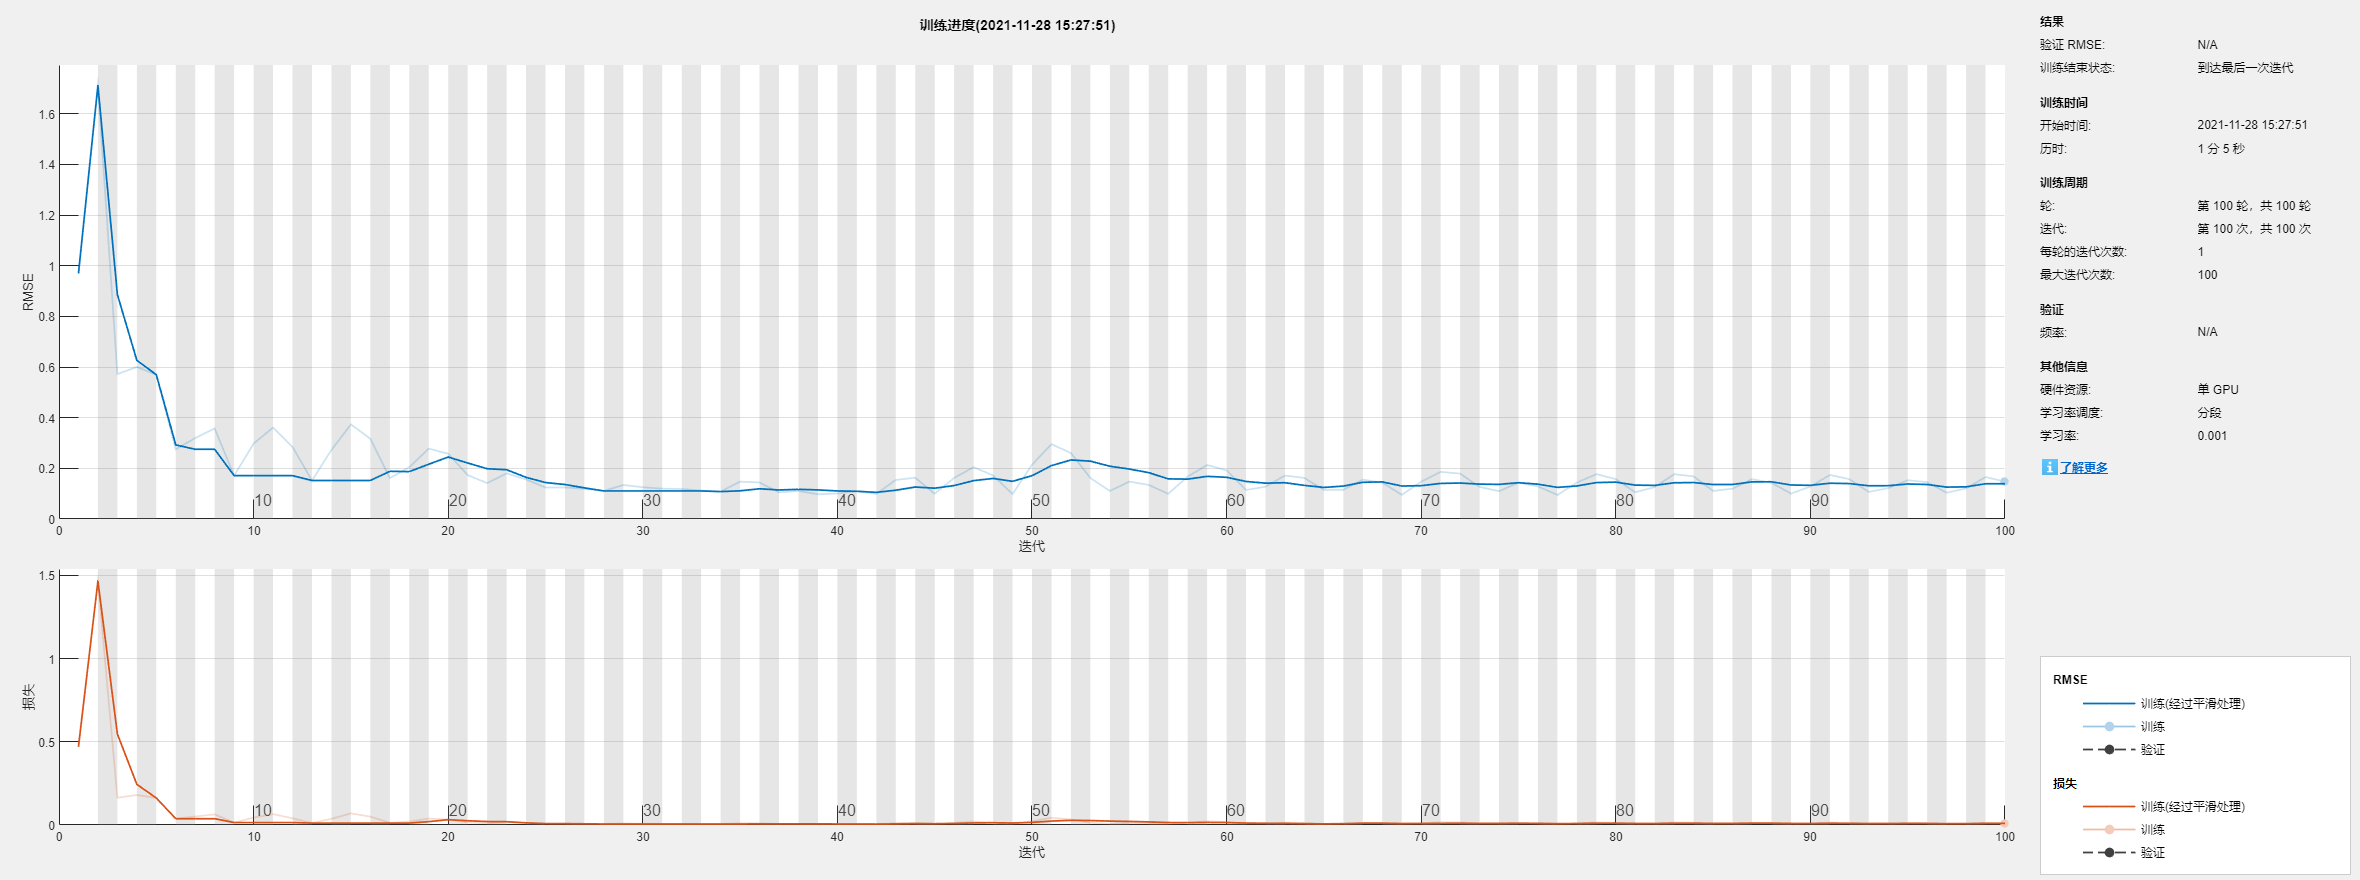
\includegraphics[width=1\linewidth]{pic/screenshot015}
		\caption{训练进度展示}
		\label{fig:screenshot015}
	\end{figure}
\end{frame}	
\begin{frame}
	\frametitle{喂入数据并训练}
	使用函数$ predict $调用训练好的模型进行预测。此神经网络预测结果如图\ref{fig:screenshot016}所示:
	
	\begin{figure}[H]
		\centering
		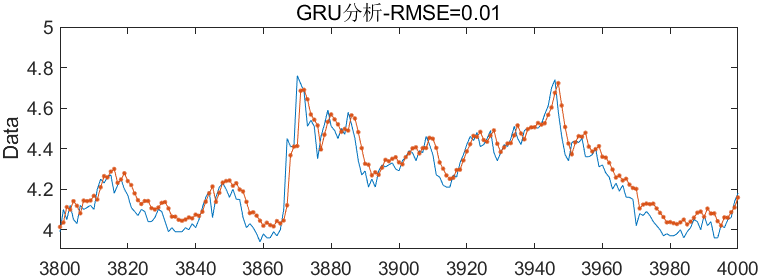
\includegraphics[width=1\linewidth]{pic/screenshot016}
		\caption{GRU预测结果:图中\textcolor[RGB]{217, 83, 25}{橘红色}曲线为预测数值, \textcolor[RGB]{97,167,212}{蓝色}为实际数值}
		\label{fig:screenshot016}
	\end{figure}
\end{frame}	
\section{模型优化}
\begin{frame}
	\frametitle{效果评判}
	后续测试模型中,我们采用茅台2005年1月1日到2021年3月20日的开盘股价作为训练集,为了节省时间,规定每一种模型均跑100Epoch。
	
	我们使用如下指标进行模型效果评判:
	\begin{itemize}
		\item 计算茅台在2021年3月30日到2021年10月16日,共计200日的开盘股价预测数据,并与此200日的实际开盘股价计算确定系数。
		
		确定系数计算公式如下:
		\begin{equation}\label{r}
			r(X,Y)=\dfrac{\texttt{Cov}(X,Y)}{\sqrt{\texttt{Var}[X]\texttt{Var}[Y]}}
		\end{equation}
		式中,$ \texttt{Cov}(X,Y) $为X与Y的协方差,$ \texttt{Var}[X] $为X的方差,$ \texttt{Var}[Y] $为Y的方差。
		\item 计算模型计算速度,测试数据为:茅台在2021年3月30日到2021年10月16日的股价预测数据。计算速度测试中,时间计算单位为ms,一共跑100次,取平均值。
	
	\end{itemize}
\end{frame}	
\begin{frame}
	\frametitle{效果评判}
	接上
	\begin{itemize}
			\item 测试设备为联想拯救者R9000P(5800H+64G内存+RTX3070-8G)
		
		\item 综合评判公式:
		
		\begin{equation}\label{pingpan}
			s=\dfrac{100r}{T}
		\end{equation}
	\end{itemize}
\end{frame}	
\begin{frame}
	\frametitle{更改模型}
	在3.3中,我们得到了粗略的结果,如图\ref{fig:screenshot005},其模型如图\ref{fig:screenshot004}。从结果中可以看出,虽然预测所得的结果趋势大致与实际情况近似,但其偏差还是较大。因此,在这一节中,我们更改了模型。其中更改的方向如下:
	
	\begin{enumerate}
		\item 增减模型层数
		\item 调整 Dropout 单元的数量和 Dropout 的数值
		\item 调整 GRU 内神经元个数
		\item 在GRU中使用 softsign 替换 tanh 
	\end{enumerate}
\end{frame}	
\begin{frame}
	\frametitle{更改模型}
	我们据此作出了10个新的模型,如表\ref{tab:my-table}所示。
	
	% Please add the following required packages to your document preamble:
	% \usepackage{graphicx}
	\begin{table}[H]
		\caption{10种调参模型}
		\label{tab:my-table}
		\resizebox{\textwidth}{!}{%
			\begin{tabular}{lll}
				\hline
				序号 & \multicolumn{1}{c}{模型结构}                                             & 备注          \\ \hline
				1  & GRU(20)→Dropout(0.2)→GRU(20)→Dropout(0.2)→Dense                      &             \\
				2  & GRU(20)→Dropout(0.2)→GRU(20)→GRU(20)→Dropout(0.2)→Dense              &             \\
				3  & GRU(40)→Dropout(0.2)→GRU(80)→Dropout(0.2)→Dense                      &             \\
				4  & GRU(20)→Dropout(0.5)→GRU(20)→Dropout(0.5)→Dense                      &             \\
				5  & GRU(80)→Dropout(0.2)→GRU(160)→Dropout(0.2)→Dense                     &             \\
				6  & GRU(20)→GRU(20)→Dropout(0.2)→Dense                                   &             \\
				7  & GRU(20)→Dropout(0.2)→GRU(20)→Dropout(0.2)→Dense                      & 输出使用softsign\\
				8  & GRU(20)→Dropout(0.7)→GRU(20)→Dropout(0.7)→Dense                      &             \\
				9  & GRU(20)→Dropout(0.2)→GRU(20)→Dropout(0.2)→GRU(20)→Dropout(0.2)→Dense &             \\
				10 & GRU(20)→Dropout(0.2)→GRU(20)→GRU(20)→GRU(20)→Dropout(0.2)→Dense      &             \\ \hline
			\end{tabular}%
		}
	\end{table}
\end{frame}	
\begin{frame}
	\frametitle{更改模型}
	下面进行模型效果评判,结果如表\ref{tab:my-table1}:
	
	%\begin{figure}[H]
	%	\centering
	%	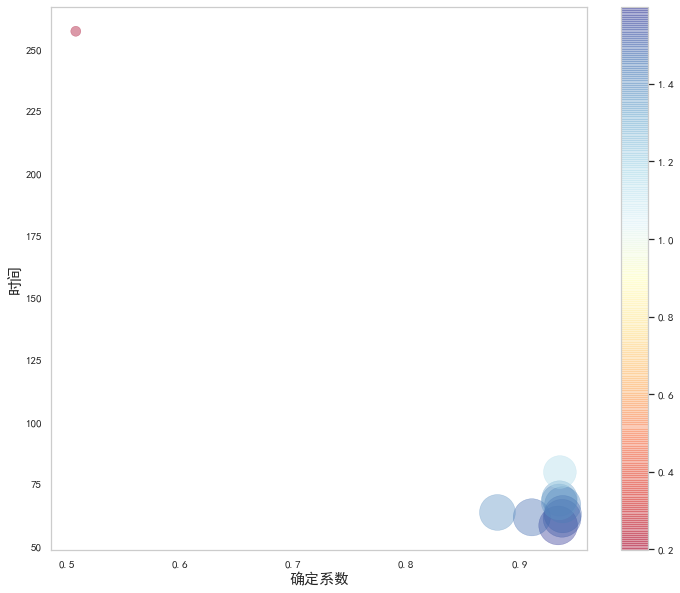
\includegraphics[width=0.7\linewidth]{pic/screenshot014}
	%	\caption{}
	%	\label{fig:screenshot014}
	%\end{figure}
	
	\begin{table}[H]
		\centering
		\caption{10种调参模型的模型效果评判}
		\label{tab:my-table1}
		\begin{tabular}{rrrrr}
			\hline
			序号& & \multicolumn{1}{c}{r} & \multicolumn{1}{c}{T / ms} & \multicolumn{1}{c}{s} \\ \hline
			1 & & 0.9342                & 58.4025               & 1.5996                \\
			2&  & 0.9354                & 69.2492               & 1.3507                \\
			3 & & 0.9376                & 61.2784               & 1.5301                \\
			4  && 0.9109                & 61.6864               & 1.4767                \\
			5  && 0.9382                & 66.7216               & 1.4061                \\
			6  && 0.9383                & 62.9502               & 1.4905                \\
			7  && 0.5082                & 257.0746              & 0.1977                \\
			8  && 0.8806                & 63.6268               & 1.3839                \\
			9  && 0.9350                & 67.8759               & 1.3776                \\
			10 && 0.9357                & 79.8768               & 1.1715                \\ \hline
		\end{tabular}
	\end{table}
\end{frame}	
\begin{frame}
	\frametitle{每个GRU单元中偏置b初始化为1}
	此处将所有偏置b初始化为1,模型代码更改为:
	\begin{figure}[H]
		\centering
		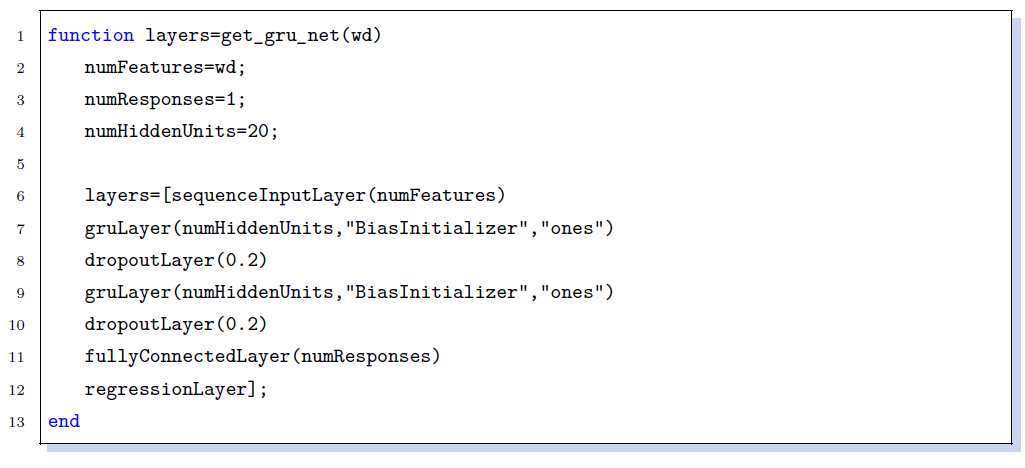
\includegraphics[width=0.7\linewidth]{pic/screenshot038}
		\label{fig:screenshot038}
	\end{figure}
	评判模型效果,结果如下:$  T=60.573ms, \ r=0.93623,\ s=\dfrac{100r}{T}=1.54562$。综合效果不如原本模型,但其训练收敛速度较原本模型有较大提升(loss收敛至$ 3\times 10^{-4} $只需要40轮)。
\end{frame}	
\begin{frame}
	\frametitle{全链接层使用Highway Network代替}
	Highway Network的灵感来自“解决RNN的问题,提出的LSTM结构”也就是加入“门”结构。
	
	对于一般网络,其输出可以用如下公式表示:
	\begin{equation}\label{normal}
		y=H(x,W^H)
	\end{equation}
	
	而在Highway Network中,我们定义一个新网络T,此时输出化为:
	
	\begin{equation}\label{HeightWay}
		y=H(x,W^H)\cdot T(x,W^T)+x\cdot (1-T(x,W^T))
	\end{equation}
\end{frame}	
\begin{frame}
	\frametitle{全链接层使用Highway Network代替}
	此时不难发现,对于特殊的T值,该输出有如式\ref{HW_Proformance}的表现:
	
	\begin{equation}\label{HW_Proformance}
		y=
		\left\{\begin{matrix} 
			x& &T=0\\  
			H&(x,W^H)\qquad\qquad&T=1
		\end{matrix}\right. 
	\end{equation}
	
	若假设所有的门T的均值为0.5的话,就是把所有的原始信息一半激活,一半不变直接输入下一层,这样一来则保留了很多信息。同时反向传播的时候,可以让更多的(梯度)信息直接回流到输入,而不需要经过一个非线性转化。
	
	由于笔者没有找到Matlab中如何自定义网络,因此此部分在Python中使用tensorflow实现。
\end{frame}	
\begin{frame}
	\frametitle{全链接层使用Highway Network代替}
	使用tensorflow定义Highway单元,其代码如下:
	\begin{figure}[H]
		\centering
		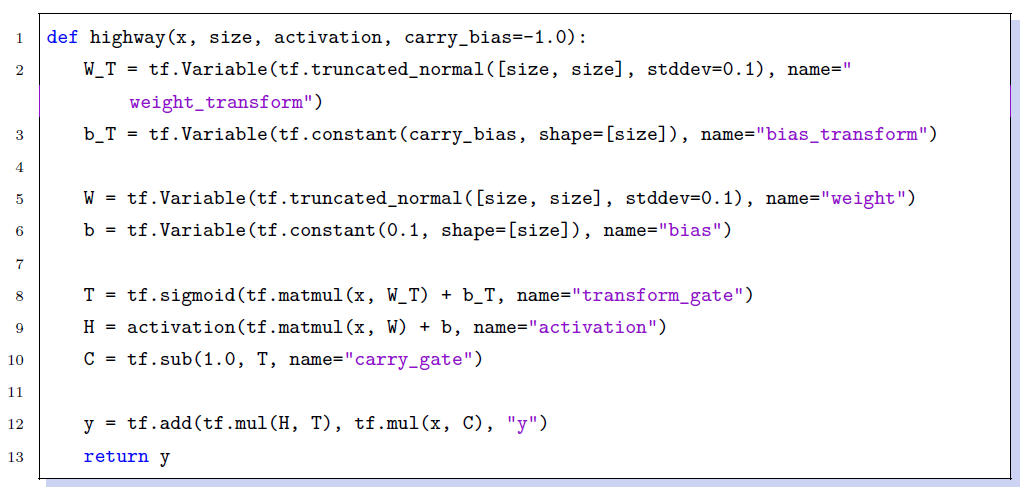
\includegraphics[width=0.7\linewidth]{pic/screenshot039}
		\label{fig:screenshot039}
	\end{figure}
	
\end{frame}	
\begin{frame}
	\frametitle{全链接层使用Highway Network代替}
	更改后的神经网络架构为:GRU(20)$ \rightarrow $Dropout(0.2)$ \rightarrow $GRU(20)$ \rightarrow $ 
	
	\noindent Dropout(0.2)$ \rightarrow $Highway   。此时对此模型进行评估可以得到如下结果:
	$  T=50.387ms, \ r=0.93382,\ s=\dfrac{100r}{T}=1.8536
	$
	
	相较于原本模型:$  T=58.402ms, \ r=0.93418,\ s=\dfrac{100r}{T}=1.5996
	$有较大幅度的提升。
\end{frame}	
\begin{frame}
	\frametitle{结果}
	由于Matlab中无法定义highway网络,因此Matlab使用结果3.4.3中模型得出结果。结果如图\ref{fig:screenshot021}所示。
	\begin{figure}[H]
		\centering
		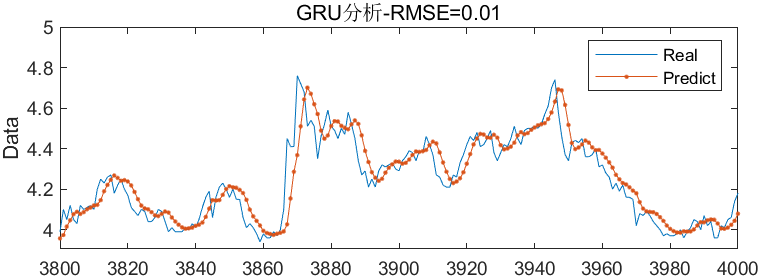
\includegraphics[width=0.8\linewidth]{pic/screenshot021}
		\caption{MATLAB中使用3.4.3中模型得出结果}
		\label{fig:screenshot021}
	\end{figure}
\end{frame}	
\begin{frame}
	\frametitle{结果}
	在Python中,把全链接层换为Highway层,得出结果如图\ref{fig:screenshot022}所示。
	\begin{figure}[H]
		\centering
		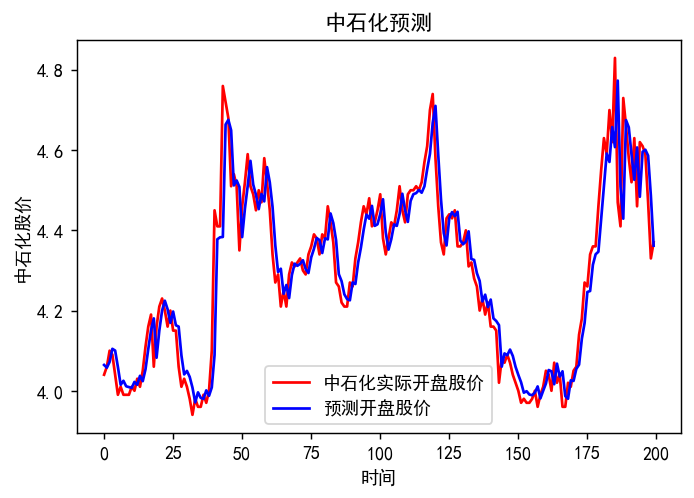
\includegraphics[width=0.5\linewidth]{pic/screenshot022}
		\caption{Python中使用3.4.4模型得出的结果}
		\label{fig:screenshot022}
	\end{figure}
	
	
\end{frame}	
\section{股市K线预测}
	
\begin{frame}
	\frametitle{K线图的画法}
	K线图源于日本,被当时日本米市的商人用来记录米市的行情与价格波动,后因其细腻独到的标画方式而被引入到股市及期货市场。下面来实现茅台预测日K线的描绘。
	\begin{figure}[H]
		\centering
		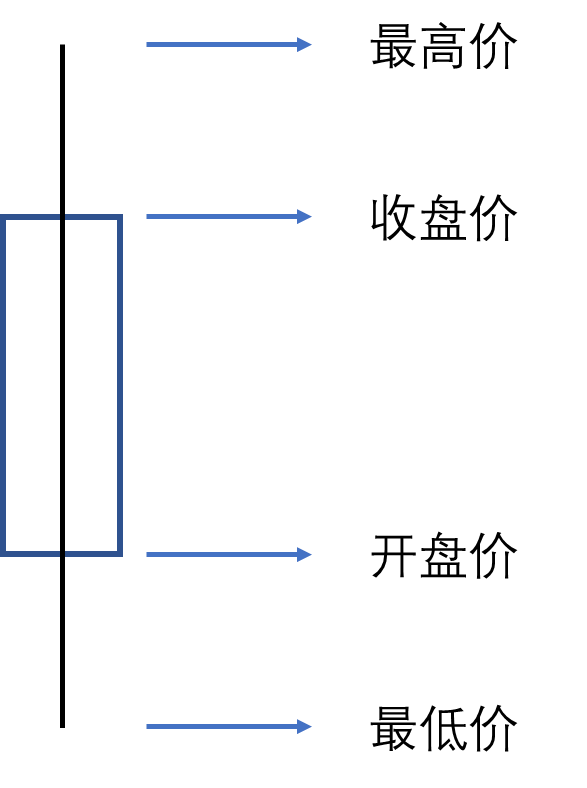
\includegraphics[width=0.2\linewidth]{pic/screenshot030}
		\caption{K线图画法}
		\label{fig:screenshot030}
	\end{figure}
\end{frame}	
\begin{frame}
	\frametitle{K线图的画法}
	
	日K线有如下特点:
	\begin{enumerate}
		\item 日K线为股票当日的开盘价、最高价、最低价、收盘价情况
		\item 阳线为红色柱体,表示股票上涨情况
		\item 阴线为绿色柱体,表示股票下跌情况
	\end{enumerate}
\end{frame}	
\begin{frame}
	\frametitle{K线数据的准备}
	K线数据需要:
	\begin{enumerate}
		\item 开盘价
		\item 最高价
		\item 最低价
		\item 收盘价
	\end{enumerate}
	
	使用上一节中的模型对此4组数据进行预测并保存到Xlsx中,方便在绘制的时候调用。
\end{frame}	
\begin{frame}
	\frametitle{Matlab中K线的实现}
	Matlab中有 candle.m函数可以实现蜡烛图的绘制,但其结果如下:
	\begin{figure}[H]
		\centering
		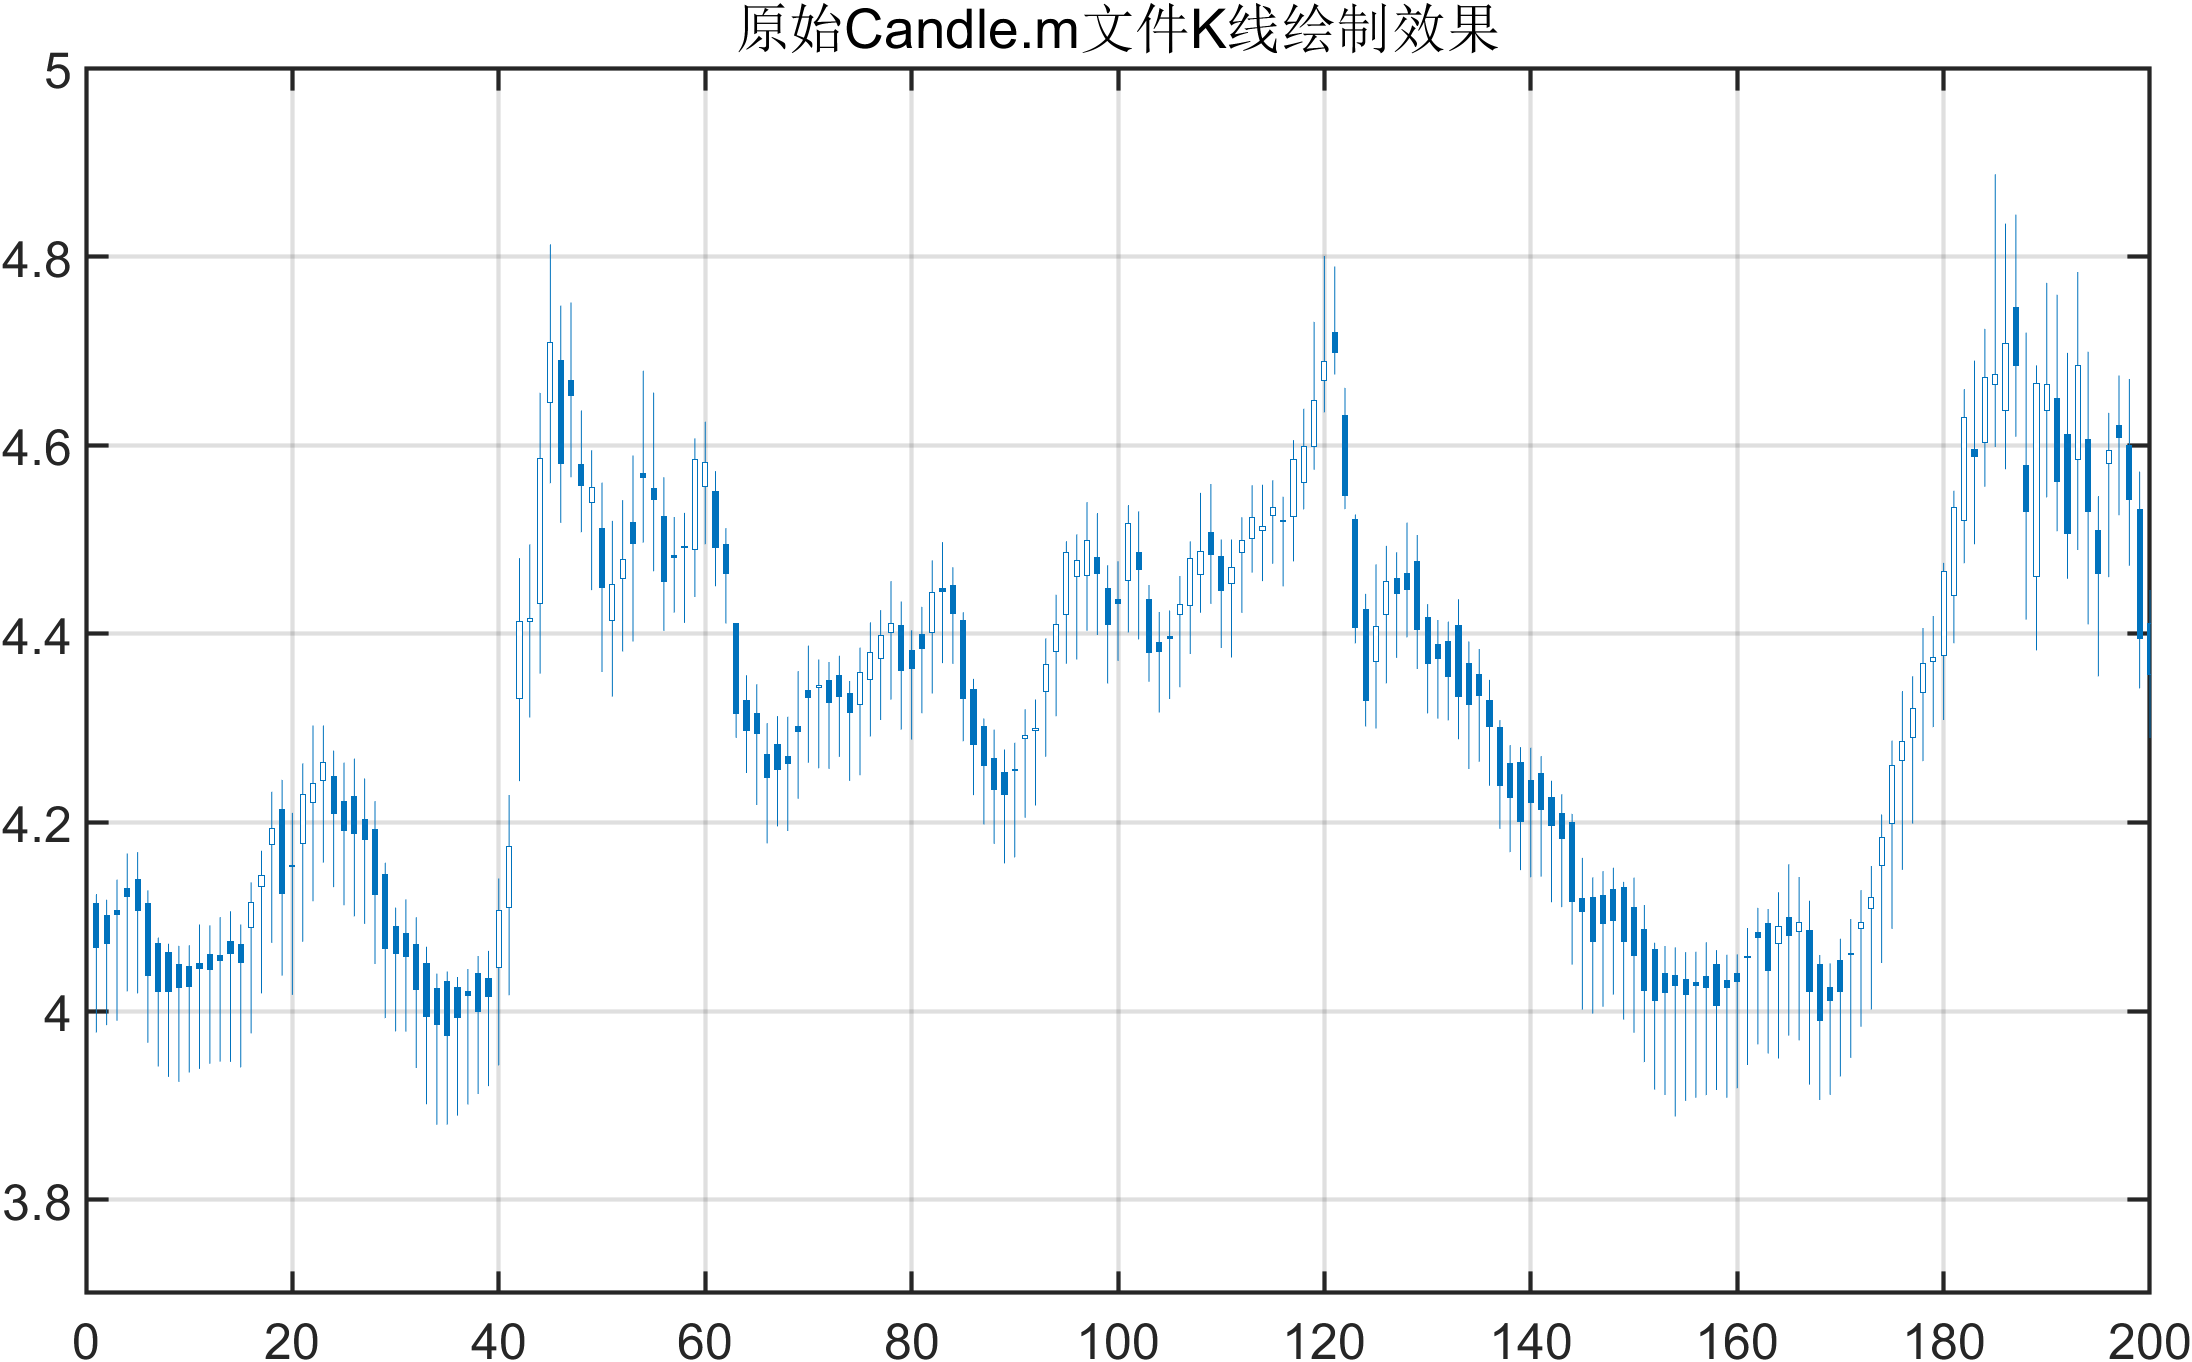
\includegraphics[width=0.4\linewidth]{pic/screenshot031}
		\caption{原始 Candle.m文件K线绘制效果}
		\label{fig:screenshot031}
		
	\end{figure}
	虽然已经有了大体的框架,但与我们常用的K线图还是有些许不同,因此需要对脚本进行修改,加入颜色,使其更加直观。
\end{frame}	
\begin{frame}
	\frametitle{结果}
\begin{figure}[H]
	\centering
	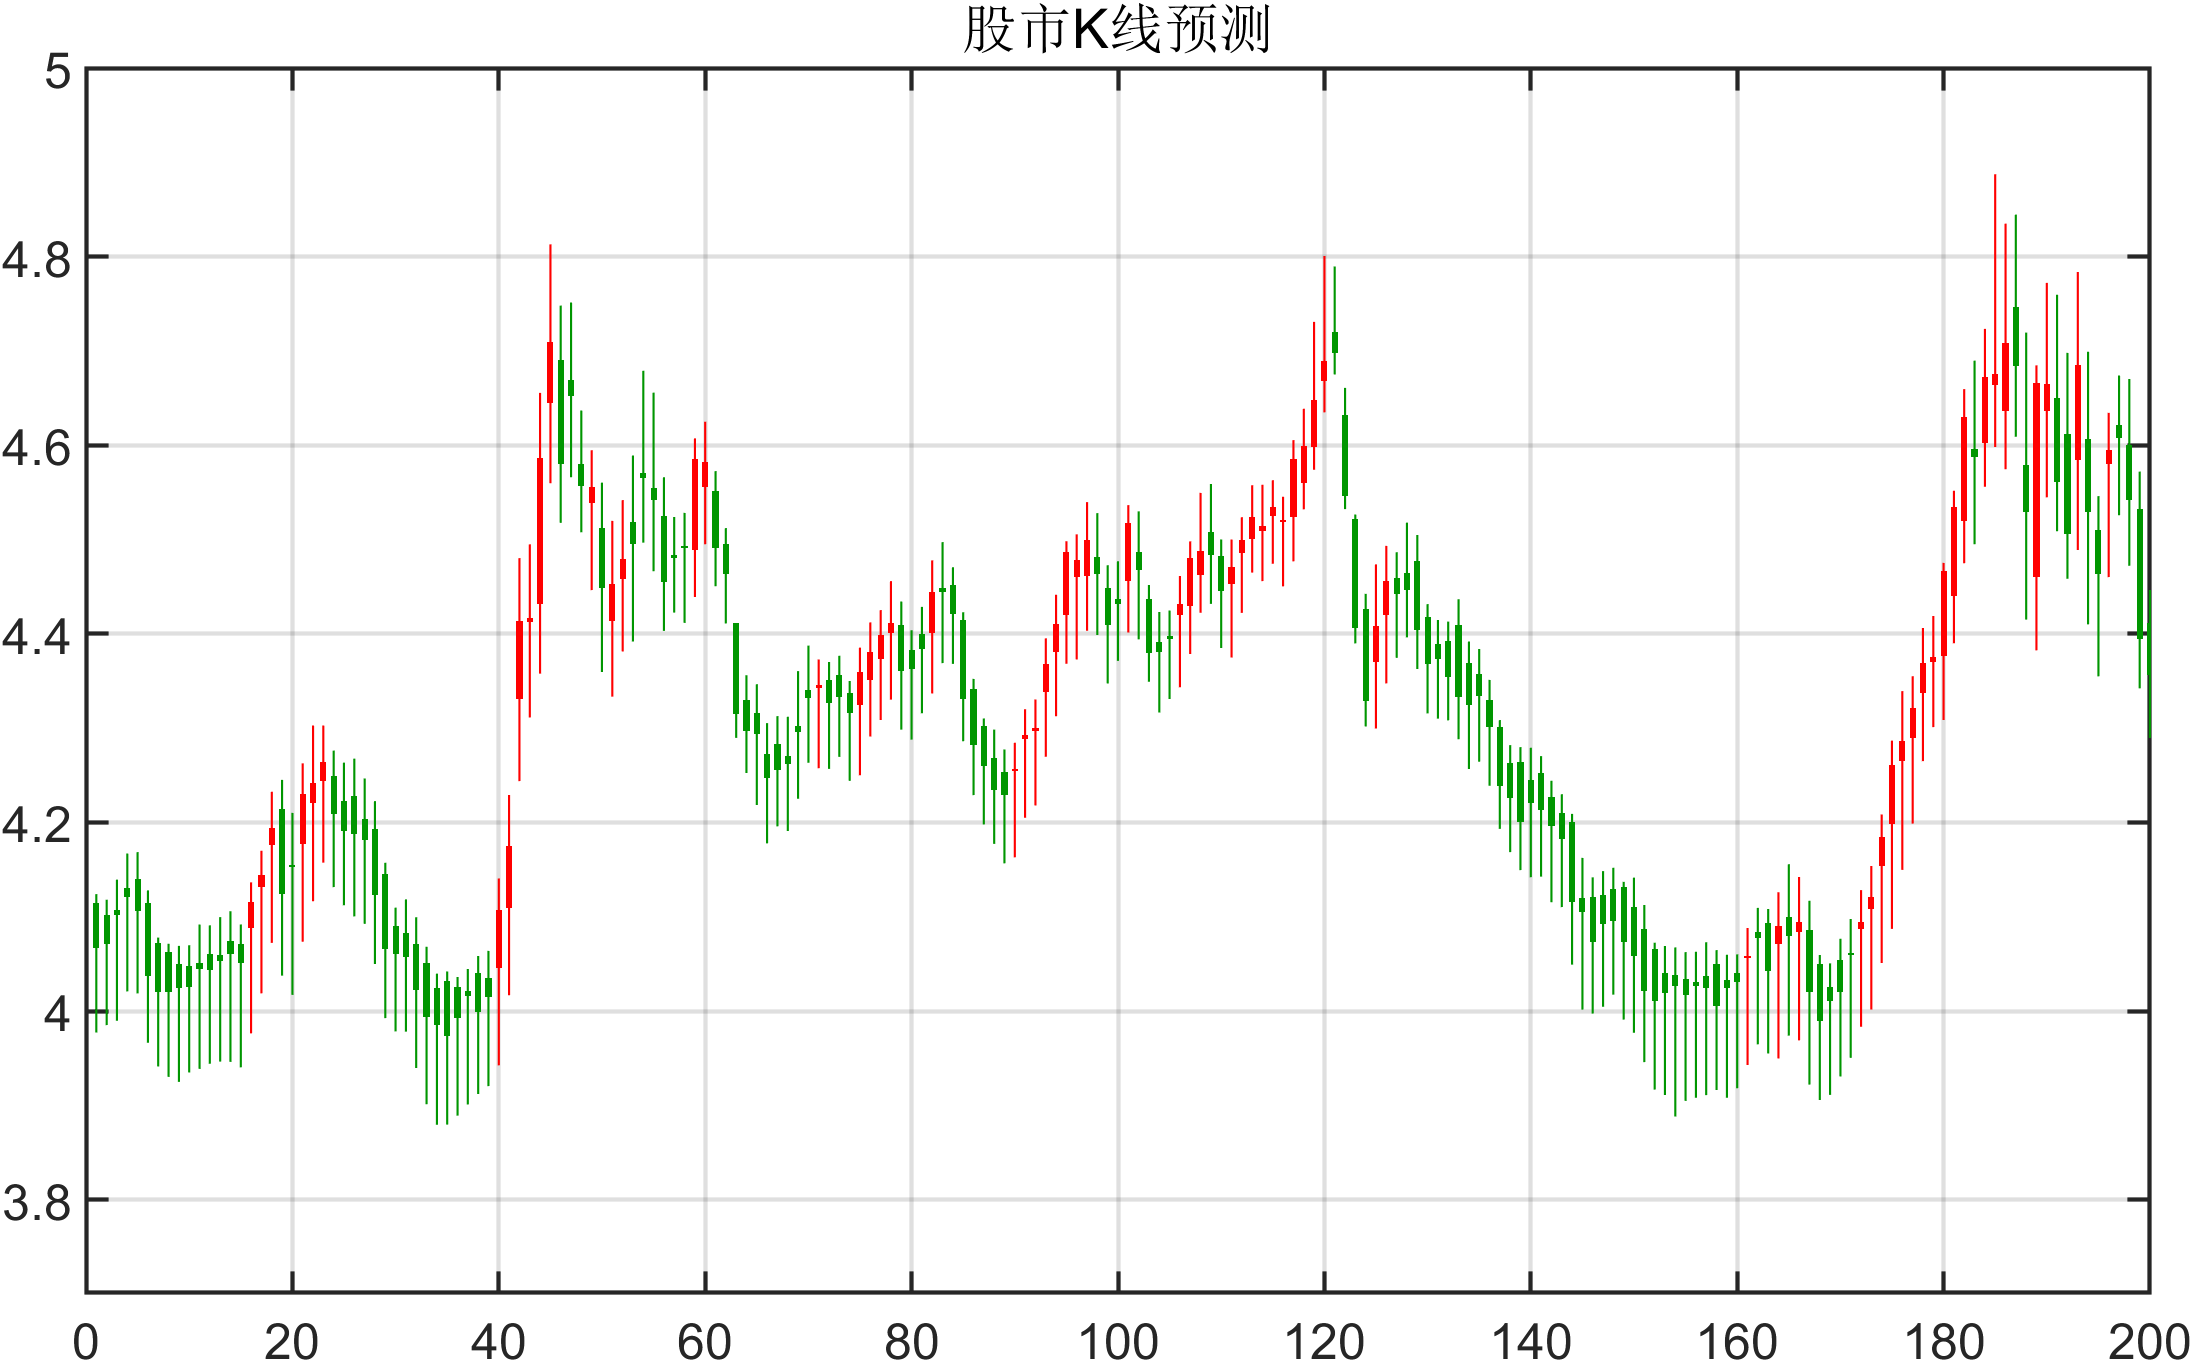
\includegraphics[width=0.65\linewidth]{pic/screenshot029}
	\caption{股市K线预测}
	\label{fig:screenshot029}
\end{figure}
\end{frame}	



	\begin{frame}
		\heiti \zihao{1}\centering{感谢聆听}
	\end{frame}
\end{document}